\begin{figure*}[htbp!]
\centering
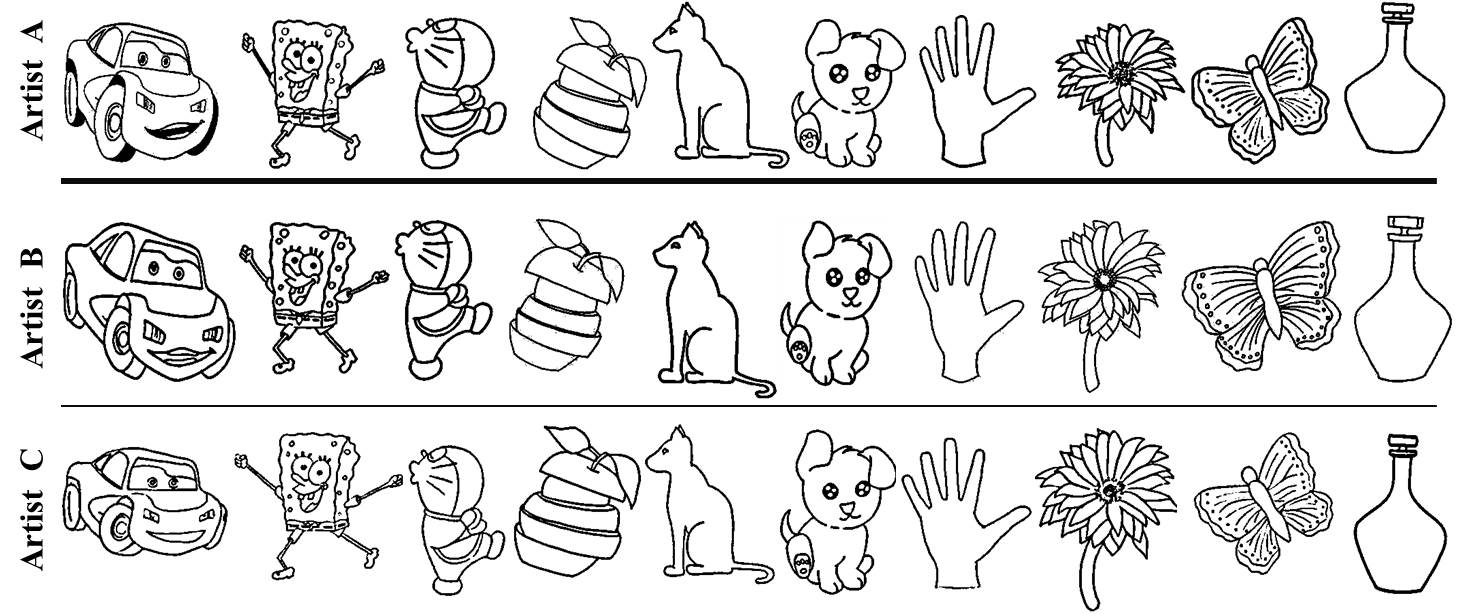
\includegraphics[width = 1.0\textwidth]{images/fraudExperiment.jpg}
\vspace{-6mm}\caption {Samples of sketches from the fraud dataset. The first row shows the original sketches drawn by Artist A. The other three rows show the sketches of 2 other artists (Artists B and C), who attempted  sketch fraud. Obviously, the \emph{fraudulent} sketches look extremely similar to the originals, making authorship recognition (manual or automatic) quite difficult.}\vspace{-5mm}
\label{FraudDataset}
\end{figure*}

For comparison and as a baseline, we study the inherent difficulty of the authorship recognition problem for humans. The human visual system (HVS) is renowned for its effectiveness in successfully completing many high-level recognition tasks (e.g. object and action recognition), so much so, that it remains the \emph{gold standard} to which automated recognition systems aspire. Despite significant advances in computer vision, the HVS almost always outperforms automated methods in such tasks. However, there \emph{do exist} recognition tasks, in which the HVS underperforms. These tasks usually deal with \emph{fine-grained} recognition of objects (e.g. faces), where the inter-class variation is minimal and on par with the intra-class variation. We motivate this fact with an example. Although the HVS can easily discriminate between a 'chair' and a 'dog', it does not do so well in recognizing a person's face in a large dataset of people (e.g. the entire population of a country) from the same cultural and racial background. The differences between people's faces are so subtle that the minute details discriminating them cannot be uncovered by the HVS. However, it is exactly these details that automated recognition methods focus on. This enables them to outperform the HVS in these tasks (e.g. robust face recognition \cite{4483511}). In this section, we provide extensive empirical evidence from two user studies that highlight the sheer difficulty people and experienced artists face when trying to recognize authorship from 2D sketches.% (similar to fine-grained face recognition).

%The first was announced to the public while the second one was targeting just a sample of the artists community. The 2 user studies are discussed in details below. Later in this paper, we will show how SAR outperforms human and artists in distinguishing the authorship and originality of sketches.

%In this section, we analyze human and artists sketch authorship recognition performance. For this purpose, we conducted 2 user studies where the first study was announced to the public while the second one was targeting just a sample of the artists community. The 2 user studies are discussed in details below. Later in this paper, we will show how SAR outperforms human and artists in distinguishing the authorship and originality of sketches.


%\vspace{-2mm}
\noindent\textbf{Authorship Recognition by Non-artists.} The aim of this study is to shed light on how accurately people can recognize sketch authorship. As an online quiz, participants are first shown sample sketches from the free style dataset labled with artists who drew them. We showed 5 randomly selected sketches from each of the 7 artists. Next, we administered for each online participant a total of 5 questions, each of which asked him/her to assign an \emph{unseen} sketch to one of the 7 artists that he/she thought drew it. We chose to show users only 5 of the 10 images per artist so as not to overwhelm them. We allowed participants to zoom-in to the images when needed. To reach a large number of participants, we published our user study on Amazon Mechanical Turk (AMT). To validate the quality and seriousness of each Turker's answers (as usually done in practise), we administer a control question at the beginning of the quiz. Moreover, Turkers are randomly directed to one of the many versions of the online study and answers from unique workers are recorded.

% This study included more than a 1000 participants.
After two months of activity and more than 2000 unique participants, the accumulated results of this study show that people can successfully recognize the authorship of a sketch (among 7 different artists) with an average accuracy of 36\% and with standard deviation of 10\%. Participants took an average of 4 minutes to complete the assigned quiz. From this result, we see that average human performance is only moderately better than a random choice classifier (i.e. choose one of the 7 artists at random irrespective of what the sketch is), which has an average accuracy of 14\% in this case. Obviously, this establishes that sketch authorship recognition is quite difficult for people. More importantly, we show later in this paper that our automated SAR approach achieves an average accuracy of 60\% under the same conditions.

%These results indicate that providing people and professionals with a tool that will assist them in distinguishing authorship of similar sketches is of an added value and an extension to an average human ability.


%\vspace{-2mm}
% might want to add that this is why fraud is hard to catch. Humans cannot even do it.
\noindent\textbf{Sketch Fraud Detection by Artists.} Similar to the previous study, but targeting artists specifically, since it is conceivable that the average person might find this task difficult due to his/her lack of sketching experience and/or artistic talent. The aim here is to evaluate the performance of artists in discriminating fraudulent sketches from original ones. A total of 25 experienced artists were given an online quiz, where 5 original and 5 fraudulent sketches were made known to each user. The sketches were taken from the fraud dataset described earlier. Each artist is then given a set of 5 recognition questions, whereby he/she needs to label the unseen sketch as original or fraud. Moreover, artists were given the chance to view their quiz results and to email us feedback. Again, not all the images in the dataset are shown to the online users so as not to overwhelm them.

The quiz results show that the artists could distinguish original sketches from fraudulent ones only 52\% of the time, as compared to 50\% random chance. Each artist took an average of 5 minutes to complete the task. As expected, most of the feedback we received elaborated on how truly difficult the task was. Later, we show that SAR significantly outperforms the artists' recognition accuracy, thus, motivating the plausibility of using SAR in an automated fraud detection system for sketches (e.g. patent drawings and cartoon sketches). We include links to both quizzes in the \textbf{supplementary material}.
%Knowing that experienced artists found such distinction difficult then we believe SAR is needed to offer a new automated solution to such a challenge.
